\documentclass[aspectratio=169,10pt]{beamer}

\usepackage[T1]{fontenc}
\usepackage[utf8]{inputenc}
\usepackage{helvet}
\usepackage{amsmath}
\usepackage{booktabs}
\usepackage{array}
\usepackage{graphicx}
\usepackage{tikz}
\usetikzlibrary{arrows.meta,positioning,calc}

\definecolor{RaceInk}{HTML}{07111F}
\definecolor{RaceNavy}{HTML}{102033}
\definecolor{RacePaper}{HTML}{F4F2EC}
\definecolor{RaceWhite}{HTML}{FEFEFC}
\definecolor{RaceCyan}{HTML}{22D3D6}
\definecolor{RaceCyanDark}{HTML}{087E89}
\definecolor{RaceAmber}{HTML}{FFB547}
\definecolor{RaceLime}{HTML}{D8FF55}
\definecolor{RaceMuted}{HTML}{687586}
\definecolor{RaceCoral}{HTML}{F47B64}

\renewcommand{\familydefault}{\sfdefault}
\setbeamertemplate{navigation symbols}{}
\setbeamercolor{normal text}{fg=RaceInk,bg=RacePaper}
\setbeamercolor{frametitle}{fg=RaceInk,bg=RacePaper}
\setbeamerfont{frametitle}{size=\fontsize{23}{25},series=\bfseries}
\setbeamersize{text margin left=.62cm,text margin right=.62cm}
\setbeamertemplate{itemize item}{\color{RaceCyanDark}$\blacktriangleright$}
\setbeamertemplate{itemize subitem}{\color{RaceAmber}$\bullet$}

\newcommand{\eyebrow}[1]{\textcolor{RaceCyanDark}{\scriptsize\bfseries\MakeUppercase{#1}}}
\newcommand{\pilot}{\tikz[baseline=-.55ex]\node[fill=RaceInk,text=RaceLime,rounded corners=3pt,inner xsep=6pt,inner ysep=3pt,font=\tiny\bfseries]{EXPLORATORY PILOT};}
\newcommand{\diagnostic}{\tikz[baseline=-.55ex]\node[draw=RaceCoral,text=RaceCoral,rounded corners=3pt,inner xsep=6pt,inner ysep=3pt,font=\tiny\bfseries]{DIAGNOSTIC ONLY};}
\newcommand{\passed}{\tikz[baseline=-.55ex]\node[fill=RaceCyanDark,text=white,rounded corners=3pt,inner xsep=6pt,inner ysep=3pt,font=\tiny\bfseries]{VALIDATED ARTIFACT};}

\setbeamertemplate{footline}{%
  \pgfmathsetlengthmacro{\progresswidth}{\paperwidth*\insertframenumber/\inserttotalframenumber}%
  \hbox{\color{RaceCyan}\rule{\progresswidth}{.7pt}}%
  \leavevmode\hbox{%
  \begin{beamercolorbox}[wd=.84\paperwidth,ht=3ex,dp=1.25ex,leftskip=.62cm]{normal text}%
    \color{RaceMuted}\tiny\bfseries AI RACE LAB \hspace{.45em}|\hspace{.45em} EVIDENCE DECK - AUGUST 2026
  \end{beamercolorbox}%
  \begin{beamercolorbox}[wd=.16\paperwidth,ht=3ex,dp=1.25ex,rightskip=.62cm plus1fil]{normal text}%
    \color{RaceMuted}\tiny\bfseries \insertframenumber\ / \inserttotalframenumber
  \end{beamercolorbox}}}

\newenvironment{darkframe}[1]{%
  \setbeamercolor{background canvas}{bg=RaceInk}%
  \setbeamercolor{normal text}{fg=white,bg=RaceInk}%
  \setbeamercolor{frametitle}{fg=white,bg=RaceInk}%
  \begin{frame}{#1}%
}{%
  \end{frame}%
  \setbeamercolor{background canvas}{bg=RacePaper}%
  \setbeamercolor{normal text}{fg=RaceInk,bg=RacePaper}%
  \setbeamercolor{frametitle}{fg=RaceInk,bg=RacePaper}%
}

\newcommand{\metric}[3]{%
\begin{tikzpicture}
\node[fill=RaceWhite,draw=RaceInk!13,rounded corners=7pt,minimum width=3.65cm,minimum height=1.48cm,align=left,text width=3.15cm,inner sep=8pt] {\textcolor{RaceCyanDark}{\tiny\bfseries #1}\\[.6mm]{\fontsize{16}{17}\selectfont\bfseries #2}\\[.2mm]{\tiny\color{RaceMuted}#3}};
\end{tikzpicture}}

\newcommand{\darkmetric}[3]{%
\begin{tikzpicture}
\node[fill=RaceNavy,draw=white!13,rounded corners=7pt,minimum width=3.65cm,minimum height=1.48cm,align=left,text width=3.15cm,inner sep=8pt] {\textcolor{RaceCyan}{\tiny\bfseries #1}\\[.6mm]{\color{white}\fontsize{17}{18}\selectfont\bfseries #2}\\[.2mm]{\tiny\color{white!55}#3}};
\end{tikzpicture}}

\newcommand{\compactmetric}[3]{%
\begin{tikzpicture}
\node[fill=RaceWhite,draw=RaceInk!13,rounded corners=7pt,minimum width=3.25cm,minimum height=1.48cm,align=left,text width=2.78cm,inner sep=7pt] {\textcolor{RaceCyanDark}{\tiny\bfseries #1}\\[.7mm]{\fontsize{15}{16}\selectfont\bfseries #2}\\[.3mm]{\tiny\color{RaceMuted}#3}};
\end{tikzpicture}}

\begin{document}

% 1
\begin{frame}[plain]
\begin{tikzpicture}[remember picture,overlay]
  \fill[RaceInk] (current page.south west) rectangle (current page.north east);
  \fill[RaceCyan] ([xshift=11.0cm]current page.south west) rectangle (current page.north east);
  \draw[RaceAmber,line width=4pt] ([xshift=11.7cm,yshift=2.25cm]current page.south west)--([xshift=15.2cm,yshift=2.25cm]current page.south west);
  \draw[RaceInk,line width=4pt] ([xshift=11.7cm,yshift=1.25cm]current page.south west)--([xshift=14.1cm,yshift=1.25cm]current page.south west);
  \node[fill=RaceAmber,text=RaceInk,rounded corners=4pt,font=\bfseries] at ([xshift=15.2cm,yshift=2.25cm]current page.south west) {U};
  \node[fill=RaceInk,text=RaceLime,rounded corners=4pt,font=\bfseries] at ([xshift=14.1cm,yshift=1.25cm]current page.south west) {S};
\end{tikzpicture}
\vspace{.35cm}
{\color{RaceCyan}\scriptsize\bfseries MULTI-AGENT LLM EVALUATION $\times$ INTERPRETABILITY}\par
\vspace{.45cm}
{\color{white}\fontsize{31}{34}\selectfont\bfseries Same game.\\Different words.\\Different behavior.}\par
\vspace{.32cm}
{\color{white!62}\large Audited pilots of strategic safety, context, and SAE steering}\par
\vfill
\pilot\hspace{.35cm}{\color{white!55}\small Qwen2.5-7B-Instruct F16 - two H100 lanes}
\end{frame}

% 2
\begin{darkframe}{The strongest result is a validity warning.}
\eyebrow{Evidence in one slide}
\vspace{.32cm}
\begin{columns}[T,onlytextwidth]
\column{.33\textwidth}\darkmetric{SURFACE}{8.4--89.2\%}{Unsafe-rate span across 18 prompt variants}
\column{.33\textwidth}\darkmetric{CONTEXT}{+34.0 pp}{largest T=0 live effect vs abstract}
\column{.33\textwidth}\darkmetric{COMPREHENSION}{FAILED}{12.5\% state update; 17.2\% terminal score}
\end{columns}
\vspace{.42cm}
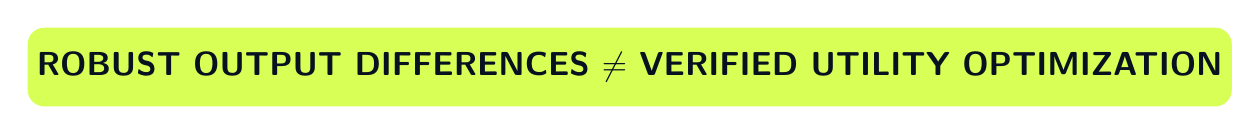
\begin{tikzpicture}
\node[fill=RaceLime,text=RaceInk,rounded corners=6pt,minimum width=14.55cm,minimum height=1.0cm,font=\large\bfseries] {ROBUST OUTPUT DIFFERENCES $\neq$ VERIFIED UTILITY OPTIMIZATION};
\end{tikzpicture}
\vfill
{\color{white!58}\scriptsize Controlled audit: one exact Qwen checkpoint. Breadth check: five pilot checkpoints under provider-specific protocols. No pooled family effect.}
\end{darkframe}

% 3
\begin{frame}{One canonical game, exact state updates.}
\eyebrow{Environment contract}\hfill\passed
\vspace{.28cm}
\begin{columns}[T,onlytextwidth]
\column{.48\textwidth}
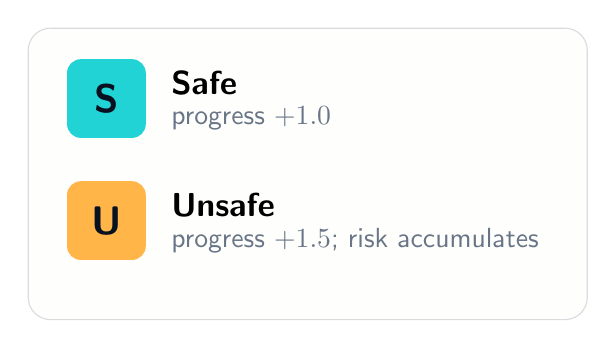
\begin{tikzpicture}
\node[fill=RaceWhite,draw=RaceInk!15,rounded corners=8pt,minimum width=7.1cm,minimum height=3.7cm] (c) {};
\node[fill=RaceCyan,text=RaceInk,rounded corners=5pt,font=\Large\bfseries,minimum size=1cm] at ($(c.north west)+(1.0,-.9)$) {S};
\node[anchor=west,font=\large\bfseries] at ($(c.north west)+(1.7,-.7)$) {Safe};
\node[anchor=west,text=RaceMuted] at ($(c.north west)+(1.7,-1.15)$) {progress $+1.0$};
\node[fill=RaceAmber,text=RaceInk,rounded corners=5pt,font=\Large\bfseries,minimum size=1cm] at ($(c.north west)+(1.0,-2.45)$) {U};
\node[anchor=west,font=\large\bfseries] at ($(c.north west)+(1.7,-2.25)$) {Unsafe};
\node[anchor=west,text=RaceMuted] at ($(c.north west)+(1.7,-2.7)$) {progress $+1.5$; risk accumulates};
\end{tikzpicture}
\column{.48\textwidth}
{\scriptsize\bfseries STAGE PAYOFF}\vspace{.08cm}
\[
\pi_i=\begin{pmatrix}1.0&0.6\\2.4&2.0\end{pmatrix},\qquad
q_i=p_{\rm risk}^{\max}\frac{n_i^U}{T}
\]
\begin{itemize}\small
\item simultaneous hidden actions; environment does arithmetic
\item minimum 5 rounds, then 20\% stop probability
\item 100-unit prize; winner/tie-specific terminal setback
\item risk caps: 10\%, 60\%, 90\%
\end{itemize}
\end{columns}
\vfill
{\color{RaceMuted}\scriptsize Adapted from Fernandez Domingos and Han (2026), arXiv:2607.26034. Human findings are not relabelled as LLM evidence.}
\end{frame}

% 4
\begin{darkframe}{Behavior is only the top layer of the audit.}
\eyebrow{Four evidence layers}
\vspace{.38cm}
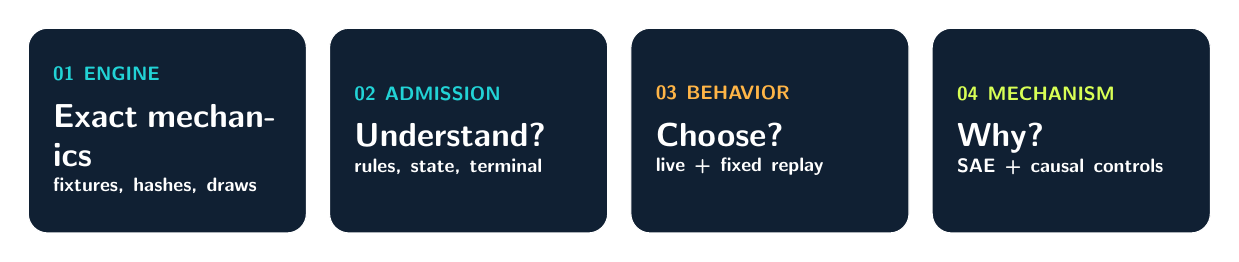
\begin{tikzpicture}[node distance=.28cm]
\tikzset{audit/.style={fill=RaceNavy,draw=white!14,rounded corners=7pt,minimum width=3.45cm,minimum height=2.6cm,text=white,align=left,text width=2.9cm,inner sep=9pt},arr/.style={-{Stealth},white!35,thick}}
\node[audit] (a) {\textcolor{RaceCyan}{\scriptsize\bfseries 01 ENGINE}\\[1mm]\large\bfseries Exact mechanics\\[-1mm]{\scriptsize\color{white!55}fixtures, hashes, draws}};
\node[audit,right=of a] (b) {\textcolor{RaceCyan}{\scriptsize\bfseries 02 ADMISSION}\\[1mm]\large\bfseries Understand?\\[-1mm]{\scriptsize\color{white!55}rules, state, terminal}};
\node[audit,right=of b] (c) {\textcolor{RaceAmber}{\scriptsize\bfseries 03 BEHAVIOR}\\[1mm]\large\bfseries Choose?\\[-1mm]{\scriptsize\color{white!55}live + fixed replay}};
\node[audit,right=of c] (d) {\textcolor{RaceLime}{\scriptsize\bfseries 04 MECHANISM}\\[1mm]\large\bfseries Why?\\[-1mm]{\scriptsize\color{white!55}SAE + causal controls}};
\draw[arr](a)--(b);\draw[arr](b)--(c);\draw[arr](c)--(d);
\end{tikzpicture}
\vspace{.48cm}
\centering{\color{RaceLime}\small\bfseries EACH LAYER HAS ITS OWN PROMOTION GATE}
\end{darkframe}

% 5
\begin{frame}{Rule recall did not transfer to game arithmetic.}
\eyebrow{Game-understanding audit}\hfill\pilot
\vspace{-.05cm}
\begin{columns}[T,onlytextwidth]
\column{.72\textwidth}

\includegraphics[width=\linewidth,height=4.55cm,keepaspectratio]{paper/figures/game_understanding_accuracy.pdf}
\column{.25\textwidth}
\metric{RAW PROBES}{685}{41 items $\times$ prompt conditions}
\vspace{.08cm}\metric{SEMANTIC}{59.1\%}{overall accuracy}
\vspace{.08cm}\metric{UNAIDED}{52.1\%}{calculator removed}
\end{columns}
\vfill
{\color{RaceMuted}\scriptsize Exact-repeat stability is narrow reliability, not an internal world model. Direct expected-payoff accuracy was 0\%.}
\end{frame}

% 6
\begin{frame}{A calculator changed play; it did not prove understanding.}
\eyebrow{Behavioral ablation}\hfill\diagnostic
\vspace{-.08cm}
\begin{columns}[T,onlytextwidth]
\column{.72\textwidth}

\includegraphics[width=\linewidth,height=4.55cm,keepaspectratio]{paper/figures/calculator_behavior_ablation.pdf}
\column{.25\textwidth}
\metric{CANONICAL}{52.0\%}{Unsafe; 558 decisions}
\vspace{.08cm}\metric{CALCULATOR}{60.8\%}{Unsafe; 558 decisions}
\vspace{.08cm}\metric{CHANGE}{+8.8 pp}{30 paired horizon cells}
\end{columns}
\vfill
{\color{RaceMuted}\scriptsize Calculator outputs demonstrate access to disclosed arithmetic. They do not identify internal causal understanding.}
\end{frame}

% 7
\begin{frame}{Five checkpoints did not share one risk-response curve.}
\eyebrow{Cross-checkpoint baseline replication}\hfill\pilot
\vspace{-.12cm}
\begin{columns}[T,onlytextwidth]
\column{.74\textwidth}

\includegraphics[width=\linewidth,height=5.08cm,keepaspectratio]{results/impact_upgrade/figures/cross_model_risk_response.pdf}
\column{.23\textwidth}
\compactmetric{BASELINE}{150 races}{2,790 decisions}
\vspace{.09cm}\compactmetric{CELL SIZE}{10 races}{per checkpoint $\times$ risk}
\vspace{.09cm}\compactmetric{INFERENCE}{SEPARATE}{no provider pooling}
\end{columns}
\vfill
{\color{RaceMuted}\scriptsize GPT-5 nano is low-flat; GPT-5.4 nano is non-monotone; three Gemini checkpoints decline with risk. This is qualitative heterogeneity, not a vendor ranking.}
\end{frame}

% 8
\begin{darkframe}{Prompt surface moved the same model across 81 points.}
\eyebrow{18-variant sensitivity grid}\hfill\pilot
\vspace{.32cm}
\begin{columns}[T,onlytextwidth]
\column{.56\textwidth}
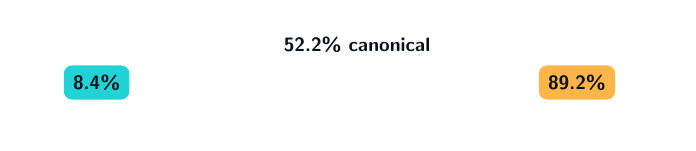
\begin{tikzpicture}[x=7.55cm]
\draw[white!22,line width=3pt] (0,0)--(1,0);
\foreach \x/\lab in {0/{0\%},.25/{25\%},.5/{50\%},.75/{75\%},1/{100\%}}{\draw[white!25](\x,-.09)--(\x,.09);\node[text=white!50,font=\tiny] at (\x,-.32){\lab};}
\node[fill=RaceCyan,text=RaceInk,rounded corners=3pt,font=\scriptsize\bfseries] at (.084,0){8.4\%};
\node[fill=white,text=RaceInk,rounded corners=3pt,font=\scriptsize\bfseries] at (.522,.48){52.2\% canonical};
\draw[white!50,dashed](.522,.12)--(.522,.36);
\node[fill=RaceAmber,text=RaceInk,rounded corners=3pt,font=\scriptsize\bfseries] at (.892,0){89.2\%};
\end{tikzpicture}
\vspace{.55cm}
{\color{white}\small\bfseries Extreme whole-trajectory variants}\par
{\color{white!62}\scriptsize action order reversed: 8.4\% Unsafe\\risk text near response: 89.2\% Unsafe}
\column{.4\textwidth}
\darkmetric{COVERAGE}{540 races}{10,044 dependent decisions}
\vspace{.12cm}\darkmetric{PARSE FAILURES}{0}{all output contracts valid}
\vspace{.12cm}\darkmetric{FIRST ROUND}{83.3\% flips}{emotional framing vs canonical}
\end{columns}
\vfill
{\color{white!55}\scriptsize Whole-trajectory differences include endogenous feedback. First-round flips compare matched initial states and seeds.}
\end{darkframe}

% 8
\begin{frame}{Eight stories preserve one mathematical game.}
\eyebrow{Context-skin invariance design}\hfill\passed
\vspace{.25cm}
\begin{columns}[T,onlytextwidth]
\column{.49\textwidth}
{\scriptsize\bfseries CONTROL SKINS}\vspace{.12cm}
\begin{itemize}\small
\item technology race
\item abstract contest
\end{itemize}
\vspace{.2cm}
{\scriptsize\bfseries REALISTIC / FICTIONAL PAIRS}\vspace{.12cm}
\begin{itemize}\small
\item logistics contract / crystal guild
\item hospital deployment / colony life support
\item robotic expedition / fictional cartography
\end{itemize}
\column{.47\textwidth}
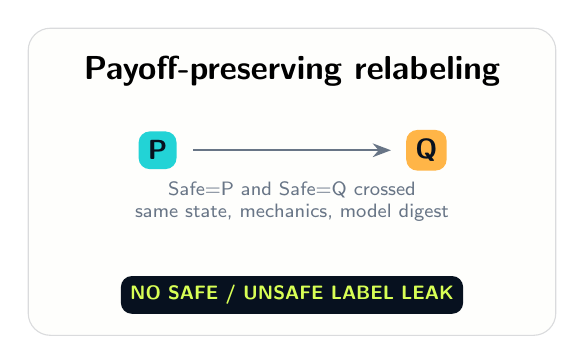
\begin{tikzpicture}
\node[fill=RaceWhite,draw=RaceInk!15,rounded corners=8pt,minimum width=6.7cm,minimum height=3.9cm,align=center] (b) {};
\node[font=\large\bfseries] at ($(b.north)+(0,-.55)$) {Payoff-preserving relabeling};
\node[fill=RaceCyan,text=RaceInk,rounded corners=4pt,font=\bfseries] at ($(b.west)+(1.65,.4)$) {P};
\node[fill=RaceAmber,text=RaceInk,rounded corners=4pt,font=\bfseries] at ($(b.east)+(-1.65,.4)$) {Q};
\draw[-{Stealth},RaceMuted,thick] ($(b.west)+(2.1,.4)$)--($(b.east)+(-2.1,.4)$);
\node[text=RaceMuted,font=\scriptsize,align=center] at ($(b.center)+(0,-.25)$) {Safe=P and Safe=Q crossed\\same state, mechanics, model digest};
\node[fill=RaceInk,text=RaceLime,rounded corners=4pt,font=\scriptsize\bfseries] at ($(b.south)+(0,.52)$) {NO SAFE / UNSAFE LABEL LEAK};
\end{tikzpicture}
\end{columns}
\vfill
{\color{RaceMuted}\scriptsize Primary: 768 live races at temperature 0; 96 engine-reachable states $\times$ 8 skins $\times$ 2 mappings at temperature 0.}
\end{frame}

% 9
\begin{frame}{Direct context response grows along live trajectories.}
\eyebrow{Fixed-state replay versus endogenous play}\hfill\diagnostic
\vspace{-.08cm}
\begin{columns}[T,onlytextwidth]
\column{.72\textwidth}

\includegraphics[width=\linewidth,height=4.92cm,keepaspectratio]{results/impact_upgrade/figures/context_direct_vs_live.pdf}
\column{.25\textwidth}
\compactmetric{ENTRY}{1,344 / 1,344}{paired actions agree}
\vspace{.07cm}\compactmetric{LIVE MAX}{+34.0 pp}{logistics vs abstract}
\vspace{.07cm}\compactmetric{DESCRIPTIVE GAP}{+18.4 pp}{live minus fixed, max}
\end{columns}
\vspace{-.1cm}
{\color{RaceMuted}\scriptsize Both protocols use T=0. Live and replay units differ: the connector is consistent with repeated exposure and feedback amplification, but is not a causal mediation estimate.}
\end{frame}

\begin{frame}{No entry flip did not mean robust trajectories.}
\eyebrow{Round-by-round divergence}\hfill\diagnostic
\vspace{-.1cm}
\begin{columns}[T,onlytextwidth]
\column{.74\textwidth}

\includegraphics[width=\linewidth,height=5.0cm,keepaspectratio]{results/impact_upgrade/figures/trajectory_divergence_curve.pdf}
\column{.23\textwidth}
\compactmetric{ROUND 1}{0 flips}{all paired contexts}
\vspace{.09cm}\compactmetric{FIRST SPLIT}{2.5--5}{conditional median round}
\vspace{.09cm}\compactmetric{CONTROL}{0}{technology divergences}
\end{columns}
\vfill
{\color{RaceMuted}\scriptsize Kaplan--Meier cumulative divergence treats race termination as censoring. Entry-only robustness checks would miss the state-conditional separation.}
\end{frame}

% 10
\begin{frame}{Opaque labels exposed a dominant code-position shortcut.}
\eyebrow{P/Q mapping diagnostic}\hfill\diagnostic
\vspace{-.12cm}
\begin{columns}[T,onlytextwidth]
\column{.74\textwidth}

\includegraphics[width=\linewidth,height=5.12cm,keepaspectratio]{results/impact_upgrade/figures/context_mapping_gate.pdf}
\column{.23\textwidth}
\compactmetric{SAFE=P}{6 / 7}{contexts diverge}
\vspace{.12cm}\compactmetric{SAFE=Q}{0 / 7}{contexts diverge}
\vspace{.12cm}\compactmetric{MAX SHIFT}{+68.0 pp}{logistics, Safe=P}
\end{columns}
\vfill
{\color{RaceMuted}\scriptsize Mapping was balanced but assigned by repetition parity. A frozen 1,536-race diagnostic now crosses both mappings inside every seed block; launch awaits current GPU NodePorts.}
\end{frame}

% 11
\begin{frame}{Temperature changes trajectories more than first moves.}
\eyebrow{Decoding robustness: T=0 versus T=0.7}\hfill\diagnostic
\vspace{-.1cm}
\begin{columns}[T,onlytextwidth]
\column{.7\textwidth}

\includegraphics[width=\linewidth,height=5.0cm,keepaspectratio]{results/open_source/context_skin_pilot/analysis_temperature_robustness/figures/context_effect_temperature_stability.pdf}
\column{.27\textwidth}
\metric{OVERALL}{+3.04 pp}{95\% CI +2.19 to +3.97}
\vspace{.08cm}\metric{ACTIONS}{88.2\%}{paired agreement}
\vspace{.08cm}\metric{TRAJECTORIES}{62.6\%}{exact player paths}
\end{columns}
\vspace{-.12cm}
{\color{RaceMuted}\scriptsize Full-effect rank $\rho=.857$; first-round delta 0.00 pp. Mechanism/template hashes and CRN horizons match, but whole staged-source hashes differ. No comprehension claim.}
\end{frame}

% 12
\begin{frame}{The context behavior study failed its admission gate.}
\eyebrow{Comprehension before interpretation}\hfill\diagnostic
\vspace{-.1cm}
\begin{columns}[T,onlytextwidth]
\column{.73\textwidth}

\includegraphics[width=\linewidth,height=5.05cm,keepaspectratio]{results/open_source/context_skin_pilot/analysis_live_pilot_t0/figures/comprehension_admission.pdf}
\column{.24\textwidth}
\metric{RULE RECALL}{100\%}{semantic accuracy}
\vspace{.1cm}\metric{STATE UPDATE}{12.5\%}{semantic accuracy}
\vspace{.1cm}\metric{TERMINAL}{17.2\%}{semantic accuracy}
\end{columns}
\vfill
{\color{RaceCoral}\scriptsize\bfseries Interpretation: prompt-conditioned action production under identical mechanics - not verified informed optimization.}
\end{frame}

% 13
\begin{darkframe}{Recognition audit v1 failed; v2 repaired the contract.}
\eyebrow{Protocol debugging is a result}
\vspace{.28cm}
\begin{columns}[T,onlytextwidth]
\column{.48\textwidth}
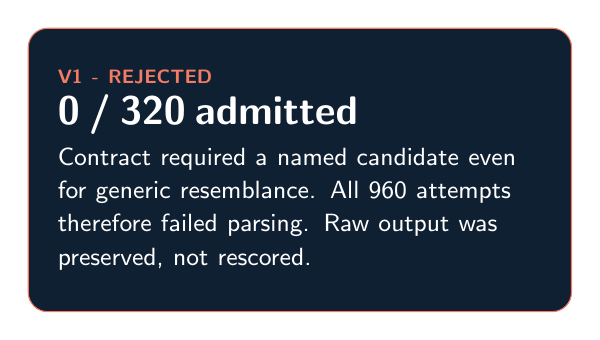
\begin{tikzpicture}
\node[fill=RaceNavy,draw=RaceCoral,rounded corners=7pt,minimum width=6.9cm,minimum height=3.6cm,align=left,text width=6.15cm,inner sep=10pt] {\textcolor{RaceCoral}{\scriptsize\bfseries V1 - REJECTED}\\[1mm]{\color{white}\Large\bfseries 0 / 320 admitted}\\[1mm]{\color{white!58}\small Contract required a named candidate even for generic resemblance. All 960 attempts therefore failed parsing. Raw output was preserved, not rescored.}};
\end{tikzpicture}
\column{.48\textwidth}
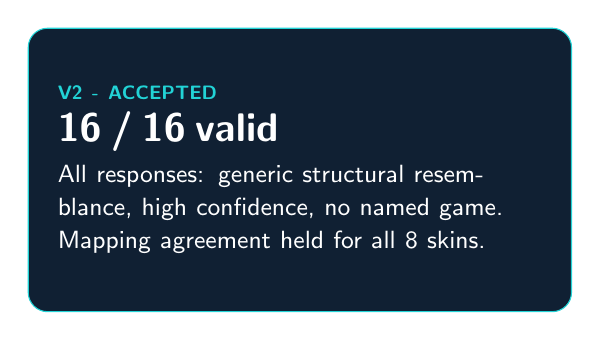
\begin{tikzpicture}
\node[fill=RaceNavy,draw=RaceCyan,rounded corners=7pt,minimum width=6.9cm,minimum height=3.6cm,align=left,text width=6.15cm,inner sep=10pt] {\textcolor{RaceCyan}{\scriptsize\bfseries V2 - ACCEPTED}\\[1mm]{\color{white}\Large\bfseries 16 / 16 valid}\\[1mm]{\color{white!58}\small All responses: generic structural resemblance, high confidence, no named game. Mapping agreement held for all 8 skins.}};
\end{tikzpicture}
\end{columns}
\vfill
{\color{white!55}\scriptsize Self-report neither proves nor rules out memorization, contamination, recognition, or latent understanding.}
\end{darkframe}

% 14
\begin{frame}{AUC answers ``decodable?'' - steering asks ``causal?''}
\eyebrow{Actual-self-play FAST-SAE design}\hfill\passed
\vspace{.33cm}
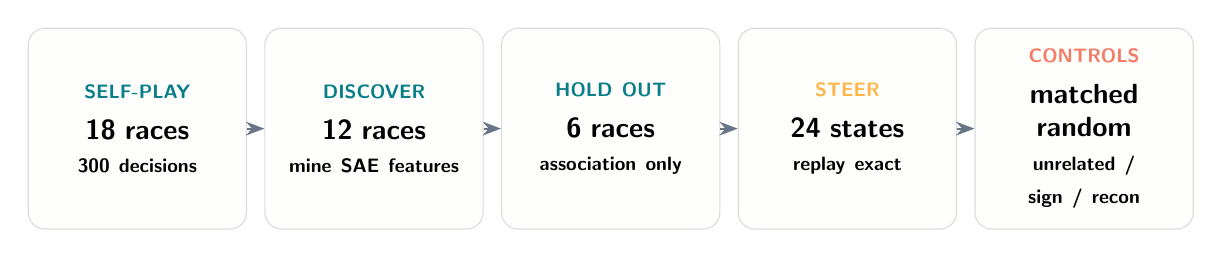
\begin{tikzpicture}[node distance=.22cm]
\tikzset{s/.style={fill=RaceWhite,draw=RaceInk!15,rounded corners=6pt,minimum width=2.75cm,minimum height=2.55cm,align=center,text width=2.35cm,inner sep=6pt},a/.style={-{Stealth},RaceMuted,thick}}
\node[s] (a) {\textcolor{RaceCyanDark}{\scriptsize\bfseries SELF-PLAY}\\[1mm]\bfseries 18 races\\{\scriptsize 300 decisions}};
\node[s,right=of a] (b) {\textcolor{RaceCyanDark}{\scriptsize\bfseries DISCOVER}\\[1mm]\bfseries 12 races\\{\scriptsize mine SAE features}};
\node[s,right=of b] (c) {\textcolor{RaceCyanDark}{\scriptsize\bfseries HOLD OUT}\\[1mm]\bfseries 6 races\\{\scriptsize association only}};
\node[s,right=of c] (d) {\textcolor{RaceAmber}{\scriptsize\bfseries STEER}\\[1mm]\bfseries 24 states\\{\scriptsize replay exact}};
\node[s,right=of d] (e) {\textcolor{RaceCoral}{\scriptsize\bfseries CONTROLS}\\[1mm]\bfseries matched random\\{\scriptsize unrelated / sign / recon}};
\draw[a](a)--(b);\draw[a](b)--(c);\draw[a](c)--(d);\draw[a](d)--(e);
\end{tikzpicture}
\vspace{.38cm}
\begin{beamercolorbox}[sep=.22cm,rounded=true]{normal text}
\small\bfseries Exact full-sequence likelihood: \texttt{ACTION: SAFE} vs \texttt{ACTION: UNSAFE}; intervention at layer 12, final prompt token.
\end{beamercolorbox}
\vfill
{\color{RaceMuted}\scriptsize Native Qwen2.5-7B-Instruct revision and FAST-SAE revision are pinned in the manifest.}
\end{frame}

% 15
\begin{frame}{Three SAE features predicted held-out actions.}
\eyebrow{Association stage}\hfill\diagnostic
\vspace{-.08cm}
\begin{columns}[T,onlytextwidth]
\column{.73\textwidth}

\includegraphics[width=\linewidth,height=5.05cm,keepaspectratio]{results/open_source/activation_sae/causal_selfplay/fast-sae-pilot-L12-v1/analysis/figures/association_selected_features.pdf}
\column{.24\textwidth}
\metric{F8505}{0.819}{held-out action AUC}
\vspace{.1cm}\metric{F16320}{0.120}{inverse-coded AUC}
\vspace{.1cm}\metric{F1803}{0.273}{inverse-coded AUC}
\end{columns}
\vfill
{\color{RaceMuted}\scriptsize Held-out absolute correlations were 0.692--0.700. Association is useful for screening; it is not a neuron-level reason.}
\end{frame}

% 16
\begin{frame}{Target steering did not beat its controls.}
\eyebrow{Fixed-state causal audit}\hfill\diagnostic
\vspace{-.12cm}
\begin{columns}[T,onlytextwidth]
\column{.73\textwidth}

\includegraphics[width=\linewidth,height=5.08cm,keepaspectratio]{results/open_source/activation_sae/causal_selfplay/fast-sae-pilot-L12-v1/analysis/figures/fixed_state_target_minus_controls.pdf}
\column{.24\textwidth}
\metric{CONTRASTS}{0 / 12}{CIs exclude zero}
\vspace{.1cm}\metric{RECON FLIPS}{12.5\%}{SAE reconstruction not neutral}
\vspace{.1cm}\metric{EVAL CLUSTERS}{6}{race-limited uncertainty}
\end{columns}
\vfill
{\color{RaceCoral}\scriptsize\bfseries No feature-specific causal-control claim. Dose curves were neither consistently monotone nor sign-reversing.}
\end{frame}

% 17
\begin{frame}{Live steering changes trajectories, then feedback takes over.}
\eyebrow{Endogenous self-play effects}\hfill\diagnostic
\vspace{-.08cm}
\begin{columns}[T,onlytextwidth]
\column{.64\textwidth}

\includegraphics[width=\linewidth,height=4.82cm,keepaspectratio]{results/open_source/activation_sae/causal_selfplay/fast-sae-pilot-L12-v1/analysis/figures/live_endogenous_payoff_effects.pdf}
\column{.33\textwidth}
\begin{itemize}\small
\item 114 live trajectories over 6 common-random-number seeds
\item direct comparable flips: 1.1--3.9\%
\item target/control action sequences matched 68.1\% on average
\item payoff deltas sit on the same scale as controls
\end{itemize}
\end{columns}
\vfill
{\color{RaceMuted}\scriptsize After the first action divergence, changed history and state make later differences total trajectory effects, not fixed-state causal effects.}
\end{frame}

% 18
\begin{frame}{Context is decodable at two layers - causality still fails.}
\eyebrow{Context FAST-SAE smoke}\hfill\diagnostic
\vspace{-.1cm}
\centering

\includegraphics[width=.96\linewidth,height=5.05cm,keepaspectratio]{results/impact_upgrade/figures/xai_decodability_vs_control.pdf}
\vfill
{\color{RaceMuted}\scriptsize Double holdout crosses unseen state trajectories and unseen context pairs ($n=56$). High AUC measures representational availability; zero held-out action flips and zero target--control intervals passing preserve the causal boundary.}
\end{frame}

% 19
\begin{frame}{Layer 20 wins the screen, not the causal claim.}
\eyebrow{Context-SAE promotion decision}\hfill\diagnostic
\vspace{-.1cm}
\begin{columns}[T,onlytextwidth]
\column{.7\textwidth}

\includegraphics[width=\linewidth,height=5.0cm,keepaspectratio]{results/open_source/activation_sae/context_fast_sae_analysis/causal_steering_controls.pdf}
\column{.27\textwidth}
\metric{LAYER 20}{PROMOTE}{capture + analysis}
\vspace{.1cm}\metric{LAYER 12}{HOLD}{smoke robustness point}
\vspace{.1cm}\metric{STEERING}{STOP}{0 held-out flips}
\end{columns}
\vfill
{\color{RaceMuted}\scriptsize Require at least 10 discovery flips before steering, or preregister continuous log-odds feature selection.}
\end{frame}

% 20
\begin{frame}{Evolution predicts a risk phase change; Qwen does not.}
\eyebrow{Reduced EGT reconstruction versus LLM self-play}\hfill\passed
\vspace{-.1cm}
\begin{columns}[T,onlytextwidth]
\column{.72\textwidth}

\includegraphics[width=\linewidth,height=5.0cm,keepaspectratio]{results/open_source/egt_reproduction/egt_theory_vs_llm_unsafe.pdf}
\column{.25\textwidth}
\metric{RISK .1 - AU}{99.2\%}{predicted Unsafe}
\vspace{.07cm}\metric{RISK .6 - CAS}{98.0\%}{predicted Unsafe}
\vspace{.07cm}\metric{RISK .9 - CS}{1.9\%}{predicted Unsafe}
\end{columns}
\vspace{-.13cm}
{\color{RaceMuted}\scriptsize Faithful, not bitwise: author code/seeds are unavailable. Official EGTTools source parity passed (transition max error $1.11\!\times\!10^{-16}$). LLM rates remain context-dependent and are not evolutionary samples.}
\end{frame}

% 21
\begin{frame}{Evidence is promoted by gates, not by effect size.}
\eyebrow{Evidence ladder}
\vspace{-.08cm}
\begin{columns}[T,onlytextwidth]
\column{.75\textwidth}

\includegraphics[width=\linewidth,height=5.08cm,keepaspectratio]{results/impact_upgrade/figures/evidence_ladder.pdf}
\column{.22\textwidth}
\compactmetric{METHOD}{VALIDATED}{engine + EGT parity}
\vspace{.1cm}\compactmetric{BEHAVIOR}{PILOT}{breadth, not population}
\vspace{.1cm}\compactmetric{MECHANISM}{WITHHELD}{controls do not pass}
\end{columns}
\vfill
{\color{RaceMuted}\scriptsize Supported: exact mechanics, localized comprehension failures, and prompt-conditioned behavior. Not supported: informed optimization, stable family effects, or a semantic Unsafe feature.}
\end{frame}

% 22
\begin{darkframe}{Promotion requires stronger controls, not more rows alone.}
\eyebrow{Next evidence grid}
\vspace{.25cm}
\begin{columns}[T,onlytextwidth]
\column{.49\textwidth}
\begin{itemize}\color{white!75}\small
\item launch frozen 1,536-race context $\times$ mapping diagnostic
\item cross both mappings within every identical live race seed
\item at least three model families and fixed decoding
\item replay logged states to separate direct effects from feedback
\end{itemize}
\column{.49\textwidth}
\begin{itemize}\color{white!75}\small
\item freeze layer, feature, sign, alpha, and controls before evaluation
\item use multiple matched-random directions as an empirical null
\item require neutral reconstruction / zero-hook gates
\item report race-level, seat-level, and strategy-level estimands together
\end{itemize}
\end{columns}
\vspace{.32cm}
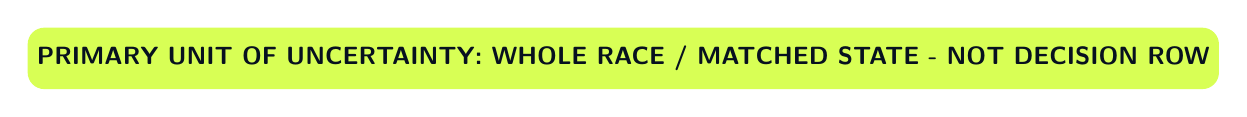
\begin{tikzpicture}
\node[fill=RaceLime,text=RaceInk,rounded corners=6pt,minimum width=14.5cm,minimum height=.78cm,font=\small\bfseries] {PRIMARY UNIT OF UNCERTAINTY: WHOLE RACE / MATCHED STATE - NOT DECISION ROW};
\end{tikzpicture}
\end{darkframe}

% 23
\begin{frame}[plain]
\begin{tikzpicture}[remember picture,overlay]\fill[RaceCyan] (current page.south west) rectangle (current page.north east);\end{tikzpicture}
\vspace{.45cm}
{\scriptsize\bfseries BOTTOM LINE}\par\vspace{.3cm}
{\fontsize{28}{31}\selectfont\bfseries Same payoff matrix.\\Different context.\\Different output.}\par
\vspace{.4cm}
{\large But the model did not pass the gate required to call that behavior informed optimization.}\par
\vspace{.52cm}

\begin{tikzpicture}[node distance=.25cm]
\tikzset{n/.style={draw=RaceInk,rounded corners=6pt,minimum width=3.2cm,minimum height=.78cm,font=\scriptsize\bfseries},a/.style={-{Stealth},RaceInk}}
\node[n] (a) {AUDIT THE GAME};\node[n,right=of a] (b) {CROSS THE WORDING};\node[n,right=of b] (c) {HOLD OUT STATES};\node[n,fill=RaceInk,text=RaceLime,right=of c] (d) {CONTROL THE CAUSE};
\draw[a](a)--(b);\draw[a](b)--(c);\draw[a](c)--(d);
\end{tikzpicture}
\vfill
{\small\bfseries Reproducible artifacts in \texttt{results/} \quad $\bullet$ \quad interactive trajectory demo + vector evidence figures}
\end{frame}

% 24
\begin{frame}{References and reproducibility.}
\eyebrow{Selected sources}\hfill\passed
\vspace{.25cm}
\begin{itemize}\small
\item Fernandez Domingos, E. and Han, T. A. (2026). \emph{Falling Behind Drives Unsafe Development in an Idealised AI Race Experiment}. arXiv:2607.26034.
\item \emph{Same Game, Different Story} (2026). Payoff-preserving contextual robustness for LLM game behavior. arXiv:2607.19670.
\item \emph{Framing the Game} (2025). Context effects in game-theoretic LLM evaluation. arXiv:2503.04840.
\item \emph{RouteSAE} (2025). Sparse autoencoders for interpreting mixture-of-experts routing. arXiv:2503.08200.
\end{itemize}
\vspace{.3cm}
\begin{beamercolorbox}[sep=.3cm,rounded=true]{normal text}
\scriptsize\ttfamily model digest: 59805ce4...ff16c\\
live context: 768 races / 13,680 decisions\\
fixed replay: 96 states / 1,536 cells\\
cross-checkpoint baseline: 150 races / 2,790 decisions\\
FAST-SAE self-play: 18 races / 300 decisions / 114 steered trajectories
\end{beamercolorbox}
\vfill
{\color{RaceMuted}\scriptsize Exact configs, raw responses, manifests, hashes, CSV summaries, PNGs, and vector PDFs are stored beside each analysis report.}
\end{frame}

\end{document}
